% ICML 2026 Preprint -- Work in Progress
% Last updated: December 2025
%
% Build with: make paper (from project root)
% See paper/WORKFLOW.md for AI agent instructions

\documentclass{article}

% Recommended packages
\usepackage{microtype}
\usepackage{graphicx}
\usepackage{subcaption}
\usepackage{booktabs}
\usepackage{hyperref}
\usepackage{amsmath,amssymb,mathtools,amsthm}
\usepackage[capitalize,noabbrev]{cleveref}
\usepackage{algorithm}
\usepackage{algorithmic}

% ICML 2026 style (preprint mode)
\usepackage[preprint]{icml2026}

% Path to figures (relative to paper/ directory, set via TEXINPUTS)
\graphicspath{{../figures/}}

%%%%%%%%%%%%%%%%%%%%%%%%%%%%%%%%
% THEOREMS AND MACROS
%%%%%%%%%%%%%%%%%%%%%%%%%%%%%%%%

\theoremstyle{plain}
\newtheorem{theorem}{Theorem}[section]
\newtheorem{proposition}[theorem]{Proposition}
\newtheorem{lemma}[theorem]{Lemma}
\newtheorem{corollary}[theorem]{Corollary}
\theoremstyle{definition}
\newtheorem{definition}[theorem]{Definition}
\newtheorem{assumption}[theorem]{Assumption}
\theoremstyle{remark}
\newtheorem{remark}[theorem]{Remark}

\newcommand{\E}{\mathbb{E}}
\newcommand{\Q}{\hat{Q}}

\icmltitlerunning{MALA-Guided Mirror Descent for Online RL}

\begin{document}

\twocolumn[
\icmltitle{MALA-Guided Mirror Descent:\\Inference-Time Q-Guidance for Diffusion Policy RL\\[0.5em]\normalsize\textit{Preprint -- Work in Progress}}

\begin{icmlauthorlist}
  \icmlauthor{Philip Nielsen}{harv}
\end{icmlauthorlist}

\icmlaffiliation{harv}{School of Engineering and Applied Sciences, Harvard University}
\icmlcorrespondingauthor{Philip Nielsen}{pnielsen@seas.harvard.edu}

\icmlkeywords{Reinforcement Learning, Diffusion Policies, Training-Free Guidance, MCMC, Langevin Dynamics}

\vskip 0.3in
]

\printAffiliationsAndNotice{}

\begin{abstract}
Diffusion policies are an expressive policy class for continuous-control reinforcement learning, but current online methods such as DPMD couple the critic tightly to training by reweighting the denoising loss with exponentiated $Q$-values.
We propose MALA-Guided Mirror Descent (MGMD), a simpler alternative that completely separates training from inference: we fit the diffusion policy by pure behavior cloning on replay actions with constant (uniform) weights, then apply $Q$-based guidance only at inference time using Metropolis-Adjusted Langevin Algorithm (MALA) corrections at each diffusion noise level.
On MuJoCo HalfCheetah-v4, MGMD achieves $14398 \pm 192$ average return (90\% CI over 5 seeds), outperforming SAC ($11114 \pm 494$) by 30\% while approaching LSAC ($17386 \pm 450$), and using constant learning rates suitable for continual learning and only a single action particle at inference time.
The clean separation between training and inference provides a simple, stable recipe for diffusion-policy RL: the diffusion loss is unweighted and stable, constant learning rates support indefinite training, and inference-time compute can be scaled independently by adjusting MALA steps or particles.
\end{abstract}

\section{Introduction}
\label{sec:intro}

Deep reinforcement learning has achieved impressive results in continuous control, yet standard Gaussian policies struggle to represent multi-modal action distributions and have no mechanism for scaling computation at inference time. In addition, ideal policy update rules must be projected back into the class of distributions with which they are defined, which is not the case for diffusion policies.
Diffusion models \citep{ho2020denoising,song2021sde} offer an appealing alternative: by learning to reverse a gradual noising process, they provide expressive policies with simple denoising score-matching losses. Using guidance, they can be flexibly repurposed for different objectives without retraining. Guidance signal can come from predictions of future rewards given partially denoised actions, allowing for scaling compute by planning at inference time as well.
Recent work has adapted diffusion models to policy learning in both offline and online RL \citep{janner2022diffuser,wang2023diffusion,ma2025soft}.

In mirror descent, the target update is 
\begin{equation}
  \pi(a\mid s) \propto \pi_\mathrm{old}(a\mid s) \exp\{\lambda Q(s,a)\}.
  \label{eq:md-tilt}
\end{equation}
Diffusion policies are typically trained with samples from the target distribution, which are not available in the online RL setting.
The Diffusion Policy Mirror Descent (DPMD) framework \citep{ma2025soft} approximately implements this update by behavior-cloning the replay buffer of its own sampled actions, reweighting by a factor of $\exp\{\lambda Q(s,a)\}$.

While effective and efficient, we note a number of ways our methods attempt to improve upon it.
First, the method relies on multiple departures from pure mirror descent in order for it to work: mainly the injection of noise in action choices and the practice of sampling the best of many action particles at inference time.
Second, implementing the update rule at training time by reweighting reduces the effective sample size compared to pure behavior cloning, potentially reducing the information learned from each transition. 
Third, the method makes no use of gradients of the critic. Better actions are only discovered if they are sampled by the base policy and up-weighted at training time. By contrast, inference time guidance uses gradients to direct sampled actions toward high-reward regions. This is expected to scale better as the dimension of the action space increases.

\paragraph{Our approach: MALA-Guided Mirror Descent (MGMD).}
We explore a complementary perspective by asking: \emph{Can we train diffusion policies with simpler, more stable objectives, and move most of the mirror-descent structure to inference time?}
MGMD cleanly separates training and inference:
\begin{enumerate}
  \item \textbf{Training:} Fit the diffusion policy by pure behavior cloning on replay actions with constant (uniform) weights. Train a standard twin Q-network via TD learning.
  \item \textbf{Inference:} Use the Q-function as an energy term to guide sampled actions toward high-value regions.
\end{enumerate}
This separation has several advantages: (i) the diffusion loss is simple and stable, with no effective-sample-size issues from importance weights; (ii) constant learning rates support continual learning without horizon-dependent schedules; (iii) inference-time compute can be scaled independently of training by adjusting the number of MALA steps or particles.

Our key finding is that constant-weight training plus MALA guidance achieves strong performance on MuJoCo benchmarks, demonstrating that the mirror-descent tilt can be implemented more accurately at inference time without sacrificing learning efficiency.

\begin{table*}[t]
  \caption{Final episode return on MuJoCo benchmarks (mean $\pm$ 90\% CI). Values are the final evaluation point of a $10^6$ step training run, where each evaluation averages 5 deterministic rollouts. Baselines from \citet{lsac2025} use 10 seeds; MGMD uses 5 seeds. CI computed via $t$-distribution. Bold indicates best. $^\dagger$ = experiments in progress.}
  \label{tab:main-results}
  \vskip 0.1in
  \begin{center}
  \begin{small}
  \begin{tabular}{lcccccccc}
    \toprule
    Environment & MGMD (Ours) & LSAC & DSAC & DIPO & SAC & TD3 & PPO & TRPO \\
    \midrule
    HalfCheetah & $14398{\scriptstyle\pm192}$ & $\mathbf{17386{\scriptstyle\pm450}}$ & $14761{\scriptstyle\pm327}$ & $11064{\scriptstyle\pm325}$ & $11114{\scriptstyle\pm494}$ & $9692{\scriptstyle\pm363}$ & $7371{\scriptstyle\pm496}$ & $7277{\scriptstyle\pm349}$ \\
    Ant & $^\dagger$ & $\mathbf{6918{\scriptstyle\pm117}}$ & $6287{\scriptstyle\pm100}$ & $5900{\scriptstyle\pm77}$ & $5385{\scriptstyle\pm328}$ & $4247{\scriptstyle\pm500}$ & $2676{\scriptstyle\pm186}$ & $3171{\scriptstyle\pm143}$ \\
    Walker2d & $^\dagger$ & $\mathbf{5910{\scriptstyle\pm197}}$ & $5672{\scriptstyle\pm276}$ & $4864{\scriptstyle\pm340}$ & $4568{\scriptstyle\pm214}$ & $4474{\scriptstyle\pm319}$ & $3208{\scriptstyle\pm120}$ & $2210{\scriptstyle\pm210}$ \\
    Hopper & $^\dagger$ & $\mathbf{3507{\scriptstyle\pm306}}$ & $3050{\scriptstyle\pm176}$ & $3071{\scriptstyle\pm171}$ & $2784{\scriptstyle\pm154}$ & $2441{\scriptstyle\pm50}$ & $1835{\scriptstyle\pm137}$ & $2023{\scriptstyle\pm145}$ \\
    Humanoid & $^\dagger$ & $8546{\scriptstyle\pm429}$ & $\mathbf{9266{\scriptstyle\pm373}}$ & $5330{\scriptstyle\pm87}$ & $6628{\scriptstyle\pm529}$ & $4620{\scriptstyle\pm313}$ & $938{\scriptstyle\pm105}$ & $3932{\scriptstyle\pm438}$ \\
    Swimmer & $^\dagger$ & $\mathbf{145{\scriptstyle\pm7}}$ & $131{\scriptstyle\pm4}$ & $113{\scriptstyle\pm6}$ & $74{\scriptstyle\pm2}$ & $102{\scriptstyle\pm6}$ & $72{\scriptstyle\pm4}$ & $58{\scriptstyle\pm3}$ \\
    \bottomrule
  \end{tabular}
  \end{small}
  \end{center}
  \vskip -0.1in
\end{table*}

\begin{figure*}[t]
  \centering
  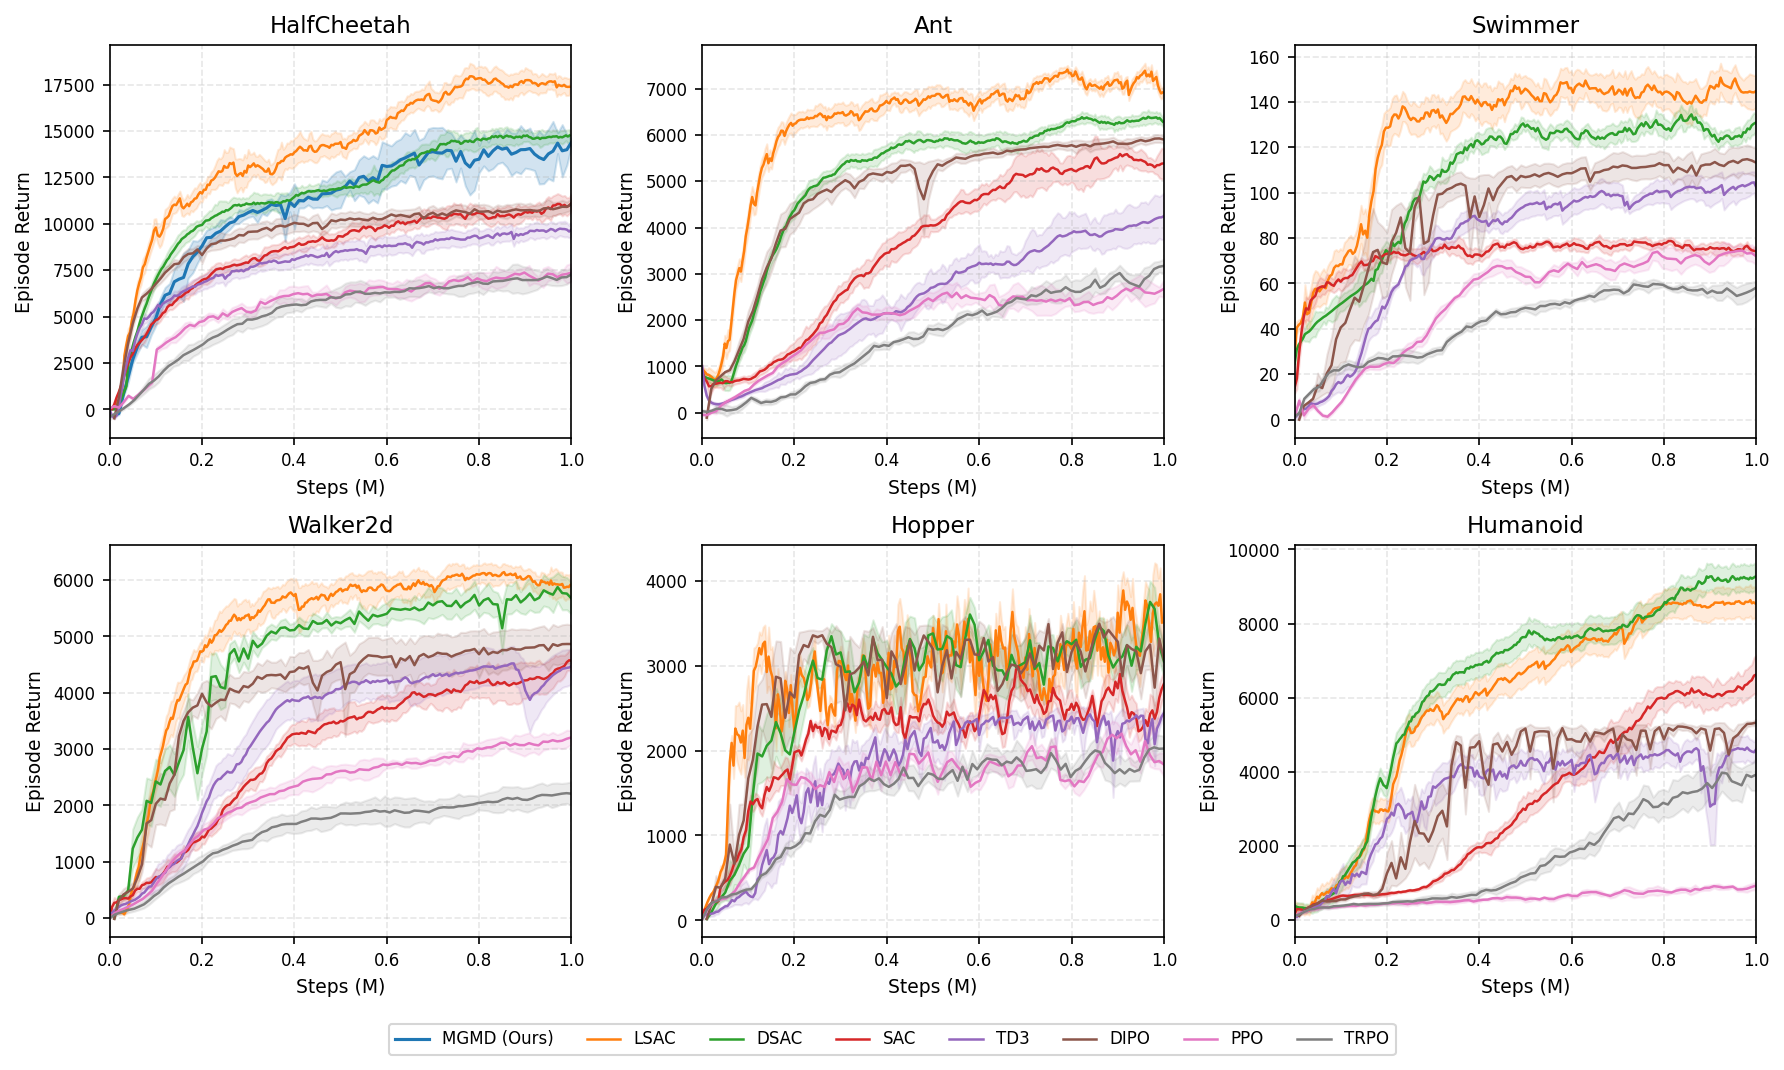
\includegraphics[width=\textwidth]{model_free_training_curves_all_envs.png}
  \caption{Training curves across 6 MuJoCo environments comparing MGMD (HalfCheetah only) against baselines from \citet{lsac2025}. Shaded regions show 90\% CI via $t$-distribution (MGMD: 5 seeds, baselines: 10 seeds).}
  \label{fig:training-curves}
  \vskip -0.1in
\end{figure*}

\section{Related Work}
\label{sec:related}

We organize our discussion of related work around the key components of our approach: diffusion models and guidance mechanisms, diffusion policies for RL, and inference-time action selection.

\paragraph{Diffusion models and guidance.}
Denoising diffusion probabilistic models (DDPMs) \citep{ho2020denoising} and score-based SDE models \citep{song2021sde} learn to reverse a gradually noised forward process.
Classifier guidance \citep{dhariwal2021beatgans} and classifier-free guidance \citep{ho2022classifierfree} modify the sampling dynamics by adding gradients of external or internal classifiers.
Training-free guidance (TFG) frameworks \citep{ye2024tfg,bansal2023universal} generalize this idea to arbitrary objectives evaluated on Tweedie-style clean estimates and highlight the need for careful treatment of guidance strength and off-manifold drift.
Energy-based diffusion with MCMC corrections \citep{du2023reduce_reuse_recycle} shows how to combine energy terms with the base diffusion model while correcting the sampler via Metropolis--Hastings steps.
These techniques have been applied primarily in image generation. In this paper, we adapt them to continuous-control RL and show that they are accurate enough to enable sample efficient online learning.

\paragraph{Diffusion policies for reinforcement learning.}
In \emph{offline} RL, Diffuser \citep{janner2022diffuser} applies trajectory-level diffusion by denoising entire state-action trajectories and conditioning on desired outcomes at inference time.
\citet{wang2023diffusion} study diffusion policies as an expressive policy class for offline continuous control, and subsequent work has explored diffusion for imitation learning and goal-conditioned control \citep{chi2023diffusion,reuss2023goal}.

In \emph{online} RL, DPMD and SDAC \citep{ma2025soft} use diffusion policies with $Q$-weighted training losses derived from a mirror-descent interpretation.
DPMD implements the tilted policy in \cref{eq:md-tilt} by reweighting the denoising loss according to exponentiated $Q$-values and selecting among a small set of denoised candidates at decision time.
Our work builds directly on DPMD but takes a different approach: we \emph{remove} $Q$ from the training loss entirely and push all mirror-descent policy improvement structure to inference time. This allows us to take advantage of the gradient of Q with repect to the action, which is not possible at training time

\paragraph{Inference-time action selection and Boltzmann policies.}
The idea of sampling actions proportionally to exponentiated $Q$-values has a long history in maximum-entropy RL.
Soft Q-learning \citep{haarnoja2017sql} and Soft Actor-Critic \citep{haarnoja2018sac} learn Boltzmann policies $\pi(a|s) \propto \exp(Q(s,a)/\tau)$ by optimizing an entropy-regularized objective.
Recent work on diffusion Q-sampling \citep{lu2024diffusionql} uses diffusion models to sample from such Boltzmann distributions in continuous action spaces.
DPMD's batch action sampling trick---generating multiple candidates and selecting based on $Q$---is a practical instantiation of this idea, though with argmax rather than stochastic selection.

Our constant-weight baseline takes this further by \emph{completely separating} the roles of training and selection: the diffusion policy is trained purely by behavior cloning with uniform weights, and all $Q$-dependent selection happens at inference time via MALA-guided sampling.
This clean separation reveals the \emph{constant-weight anomaly}: in our setting, most of the performance benefit attributed to $Q$-reweighted training in DPMD actually comes from inference-time selection.

\paragraph{Langevin dynamics in RL.}
Langevin dynamics has been used in RL for both policy sampling and critic learning.
Soft Q-learning \citep{haarnoja2017sql} uses Stein Variational Gradient Descent to sample from Boltzmann policies.
LSAC \citep{lsac2025} applies Langevin dynamics to the critic parameters themselves, using SGLD noise in Q-network updates to maintain epistemic uncertainty for exploration.
Our approach differs in that we apply MALA to the \emph{action space} during diffusion sampling, using Langevin dynamics to guide the reverse process toward high-Q regions rather than to maintain uncertainty in the critic.
MGMD is purely model-free. We do not learn or use any dynamics model.

\section{Background}
\label{sec:background}

We briefly summarize the base DPMD setup and training-free guidance from a mathematical perspective.

\subsection{Diffusion policies and DPMD}

We parameterize the policy as a conditional diffusion model $\pi_\theta(a\mid s)$ together with twin Q-functions $Q_1,Q_2$.
A fixed forward process progressively adds Gaussian noise to a clean action $a_0$ to obtain $a_T$, and a reverse process learns to denoise $a_T$ back to $a_0$ via denoising score matching.

DPMD implements a mirror-descent-style policy update by combining off-policy TD learning for $Q_1,Q_2$ with a \emph{weighted} denoising loss for the policy.
The diffusion loss takes the form
\begin{equation}
  \mathcal{L}_{\text{diff}} = \E\big[ w(s,a) \; \| \epsilon_\theta(a_t,s,t) - \epsilon \|^2 \big],
\end{equation}
where $a$ is the clean replay action and $w(s,a)$ is derived from a standardized version of $Q_{\min}(s,a) = \min(Q_1,Q_2)$.
In the original implementation the running mean $m$ and standard deviation $\sigma$ of $Q_{\min}$ are tracked and scores are clipped, exponentiated, and renormalized to keep the \emph{effective sample size} of the weights close to the batch size.

At inference time, DPMD draws $N$ action candidates from the policy and selects the argmax under $Q_{\min}$.

\subsection{Training-free guidance and Tweedie estimates}

Training-free guidance (TFG) \citep{ye2024tfg,bansal2023universal} views guidance as composing an energy term $\lambda J(s,a)$ with the base diffusion model and adjusting the reverse process accordingly.
Given a noisy action $a_t$ and a learned noise predictor $\epsilon_\theta(a_t,s,t)$, Tweedie's formula provides an estimate of the clean action
\begin{equation}
  \hat{a}_0 = \frac{a_t - \sqrt{1-\bar{\alpha}_t}\, \epsilon_\theta(a_t,s,t)}{\sqrt{\bar{\alpha}_t}},
\end{equation}
where $\bar{\alpha}_t$ is the cumulative product of $(1-\beta_t)$ along the noise schedule.
A simple TFG update modifies the noise prediction as
\begin{equation}
  \epsilon_{\text{guided}} = \epsilon_\theta - \lambda \sigma_t \nabla_{a_t} J(s,\hat{a}_0(a_t)),
\end{equation}
which heuristically moves samples toward decreasing energy $J$.
However, this modification alone does not guarantee sampling from the correctly tilted distribution.

\section{Methods}
\label{sec:methods}

We develop our MALA-guided approach by first establishing the connection between diffusion training and score functions, then showing how guidance modifies the target distribution, and finally explaining why MCMC corrections are necessary for accurate sampling.

\subsection{Diffusion training as score matching}
\label{sec:score-matching}

The standard diffusion training objective is intimately connected to score function estimation.
Consider the forward noising process that corrupts a clean action $a_0$ to a noisy version $a_t = \sqrt{\bar{\alpha}_t}\, a_0 + \sqrt{1-\bar{\alpha}_t}\, \epsilon$ where $\epsilon \sim \mathcal{N}(0,I)$ and $\bar{\alpha}_t = \prod_{i=1}^t (1-\beta_i)$ is the cumulative noise schedule.
The denoising score matching objective trains a network $\epsilon_\theta$ to predict the noise:
\begin{equation}
  \mathcal{L}_{\text{DSM}} = \E_{a_0, \epsilon, t}\bigl[\|\epsilon_\theta(a_t, s, t) - \epsilon\|^2\bigr].
  \label{eq:dsm}
\end{equation}
This objective is equivalent to learning the score function $\nabla_{a_t} \log p_t(a_t \mid s)$ of the noisy marginal distribution.
Specifically, the optimal noise predictor satisfies
\begin{equation}
  \epsilon_\theta^*(a_t, s, t) = -\sqrt{1-\bar{\alpha}_t}\, \nabla_{a_t} \log p_t(a_t \mid s),
  \label{eq:score-noise}
\end{equation}
so that learning to denoise is equivalent to learning the score.
This score-based interpretation is central to understanding how guidance modifies the sampling distribution.

\subsection{From classifier guidance to energy guidance}
\label{sec:classifier-guidance}

Suppose we wish to sample from a tilted distribution $\tilde{p}_0(a_0 \mid s) \propto p_0(a_0 \mid s) \exp\{\lambda J(s, a_0)\}$ for some objective $J$ (in our case, $J = Q$).
Standard DDPM/DDIM sampling generates samples from $p_0$ by iteratively applying the learned score.
To sample from the tilted distribution $\tilde{p}_0$, we need the score of the corresponding noisy marginals $\tilde{p}_t$.

\paragraph{Classifier guidance with noisy classifiers.}
The original classifier guidance approach \citep{dhariwal2021beatgans} observes that if we have access to a classifier $p(y \mid a_t)$ trained on \emph{noisy} inputs, then by Bayes' rule:
\begin{equation}
  \nabla_{a_t} \log p_t(a_t \mid y) = \nabla_{a_t} \log p_t(a_t) + \nabla_{a_t} \log p(y \mid a_t).
  \label{eq:classifier-guidance}
\end{equation}
This gives the exact score for conditional generation, and standard DDPM sampling with the modified score produces samples from the correct conditional distribution.
However, this approach requires training a classifier on noisy data at each noise level, which is expensive and often produces weak gradients---the classifier must distinguish between heavily corrupted inputs, yielding noisy guidance signals.

\paragraph{Training-free guidance via Tweedie estimates.}
To avoid training noise-conditional classifiers, training-free guidance (TFG) methods \citep{ye2024tfg,bansal2023universal} instead evaluate the objective on a \emph{clean estimate} obtained via Tweedie's formula:
\begin{equation}
  \hat{a}_0(a_t) = \frac{a_t - \sqrt{1-\bar{\alpha}_t}\, \epsilon_\theta(a_t, s, t)}{\sqrt{\bar{\alpha}_t}}.
  \label{eq:tweedie}
\end{equation}
The guidance gradient is then computed as $\nabla_{a_t} J(s, \hat{a}_0(a_t))$, which benefits from evaluating $J$ (e.g., a Q-function) on clean action estimates rather than noisy inputs.
This yields much stronger guidance signals since $J$ is trained on clean data.

The TFG update modifies the noise prediction as:
\begin{equation}
  \epsilon_{\text{guided}} = \epsilon_\theta - \lambda \sqrt{1-\bar{\alpha}_t}\, \nabla_{a_t} J(s, \hat{a}_0(a_t)).
  \label{eq:tfg-update}
\end{equation}
Intuitively, this steers the denoising trajectory toward regions of high $J$.

\subsection{Why Tweedie-based guidance requires MCMC}
\label{sec:why-mcmc}

Despite its practical effectiveness, Tweedie-based guidance fundamentally changes the nature of the sampling problem in a way that breaks the guarantees of standard diffusion sampling.

\paragraph{The distribution mismatch.}
Let $\tilde{p}_0(a_0 \mid s) \propto p_0(a_0 \mid s) \exp\{\lambda J(s, a_0)\}$ be our target tilted distribution.
For standard DDPM sampling to produce exact samples from $\tilde{p}_0$, the reverse process would need to follow the score of the \emph{noisy} tilted marginals $\tilde{p}_t(a_t \mid s)$.
These marginals are defined by the forward process applied to $\tilde{p}_0$:
\begin{equation}
  \tilde{p}_t(a_t \mid s) = \int p_{t|0}(a_t \mid a_0)\, \tilde{p}_0(a_0 \mid s)\, da_0.
  \label{eq:tilted-marginal}
\end{equation}
The score of this distribution is not simply the base score plus a guidance term.
Specifically, while we have $\nabla_{a_0} \log \tilde{p}_0 = \nabla_{a_0} \log p_0 + \lambda \nabla_{a_0} J$ at $t=0$, this additive decomposition does not hold for $t > 0$:
\begin{equation}
  \nabla_{a_t} \log \tilde{p}_t(a_t) \neq \nabla_{a_t} \log p_t(a_t) + \lambda \nabla_{a_t} J(s, \hat{a}_0(a_t)).
  \label{eq:score-mismatch}
\end{equation}
The TFG update \cref{eq:tfg-update} therefore does not correspond to the reverse process of any well-defined forward diffusion.

\paragraph{A sequence of energy-based targets.}
Nevertheless, the TFG-modified score does define a meaningful sequence of distributions.
Following \citet{du2023reduce_reuse_recycle}, we can interpret the guided sampler as targeting a sequence of energy-based distributions:
\begin{equation}
  q_t(a_t \mid s) \propto \exp\bigl\{-E_t(a_t, s)\bigr\},
  \label{eq:energy-sequence}
\end{equation}
where the composite energy at level $t$ is
\begin{equation}
  E_t(a_t, s) = -\log p_t(a_t \mid s) - \lambda J(s, \hat{a}_0(a_t)).
  \label{eq:composite-energy}
\end{equation}
These distributions $q_t$ smoothly interpolate from a nearly Gaussian distribution at $t=T$ (where the guidance term has little effect) to the desired tilted policy $\tilde{p}_0$ at $t=0$ (where $\hat{a}_0 \approx a_0$).

\paragraph{The sampling gap.}
The critical issue is that even if our samples $a_t$ at some noise level are distributed according to $q_t$, a single guided DDPM step does \emph{not} guarantee that the resulting $a_{t-1}$ will be distributed according to $q_{t-1}$.
The DDPM update was derived as the time-reversal of the OU forward process, but the sequence $\{q_t\}$ does not arise from any such forward process.
Consequently, guided DDPM sampling accumulates errors across noise levels.

\subsection{MALA-corrected sampling}
\label{sec:mala}

To bridge the gap between the guided dynamics and the target distributions $\{q_t\}$, we employ Markov Chain Monte Carlo (MCMC) corrections at each noise level.
Specifically, we use the Metropolis-Adjusted Langevin Algorithm (MALA), which combines gradient-based proposals with Metropolis--Hastings (MH) acceptance to ensure asymptotically exact sampling from a target distribution defined by an energy function.

\paragraph{Energy-based parameterization.}
To enable MH corrections, we require the ability to evaluate the energy $E_t$ (not just its gradient).
We therefore use an \emph{energy-based parameterization} of the diffusion policy: instead of directly outputting noise predictions, the network outputs a scalar energy $E_\theta(a_t, s, t)$, and the score is obtained by automatic differentiation:
\begin{equation}
  \nabla_{a_t} \log p_\theta(a_t \mid s, t) = -\nabla_{a_t} E_\theta(a_t, s, t).
  \label{eq:energy-param}
\end{equation}
Training proceeds by the standard denoising objective, but the energy-based form allows us to compute acceptance probabilities for MCMC.

\paragraph{Composite energy for Q-guidance.}
At each diffusion level $t$, we define the total energy that combines the learned prior with the Q-function:
\begin{equation}
  E_t^{\text{total}}(a_t, s) = E_\theta(a_t, s, t) - \lambda Q(s, \hat{a}_0(a_t)),
  \label{eq:total-energy}
\end{equation}
where $\hat{a}_0(a_t)$ is the Tweedie estimate \cref{eq:tweedie} and $Q$ is the aggregated critic (mean of $Q_1, Q_2$ in our implementation).
The corresponding Boltzmann distribution $q_t(a_t) \propto \exp\{-E_t^{\text{total}}(a_t, s)\}$ is our target at level $t$.

\paragraph{MALA corrector steps.}
At each diffusion level, after the standard DDPM predictor step, we apply $K$ MALA corrector steps to bring the sample distribution closer to $q_t$.
A single MALA step proposes:
\begin{equation}
  a_t' = a_t - \eta_t \nabla_{a_t} E_t^{\text{total}}(a_t, s) + \sqrt{2\eta_t}\, z, \quad z \sim \mathcal{N}(0, I),
  \label{eq:mala-proposal}
\end{equation}
and accepts with probability
\begin{equation}
  \alpha = \min\Bigl(1, \frac{q_t(a_t') \, \mathcal{T}(a_t \mid a_t')}{q_t(a_t) \, \mathcal{T}(a_t' \mid a_t)}\Bigr),
  \label{eq:mh-accept}
\end{equation}
where $\mathcal{T}(a' \mid a) = \mathcal{N}(a' ; a - \eta \nabla E, 2\eta I)$ is the proposal kernel.

\paragraph{Adaptive step sizes.}
Following \citet{RobertsTweedie1996MALA}, the optimal acceptance rate for MALA in high dimensions is approximately $0.574$.
We maintain a separate log-step-size $\log \eta_t$ for each diffusion level and adapt via Robbins--Monro updates:
\begin{equation}
  \log \eta_t \leftarrow \log \eta_t + \alpha_{\text{adapt}} \bigl(\text{accept\_rate}_t - 0.574\bigr),
  \label{eq:eta-adapt}
\end{equation}
with $\alpha_{\text{adapt}} = 0.2$.
Per-level adaptation is essential: the energy landscape is smooth at high noise (large $t$, requiring larger steps) and sharp at low noise (small $t$, requiring smaller steps).

\paragraph{Complete sampling procedure.}
The full MGMD sampler interleaves DDPM predictor steps with MALA corrector steps.
At each level $t$, we:
\begin{enumerate}
  \item Apply $K_{\text{MALA}}$ corrector steps targeting $q_t$, adapting $\eta_t$.
  \item Apply a guided DDPM predictor step: the noise prediction is modified by $\nabla_{a_t} Q$ to yield $a_{t-1}$.
\end{enumerate}
This predictor-corrector structure, inspired by \citet{du2023reduce_reuse_recycle}, ensures that samples approximately follow the sequence of tilted distributions while the predictor provides efficient transitions between noise levels.

\paragraph{Relation to prior work.}
Our approach builds directly on the compositional diffusion framework of \citet{du2023reduce_reuse_recycle}, which showed that MCMC corrections are necessary for accurate compositional generation in image domains.
We adapt their insights to continuous-control RL, using the Q-function as the guidance energy.
Compared to training-free guidance methods \citep{ye2024tfg,bansal2023universal} that modify the score without MH correction, MALA provides asymptotic guarantees on the sampling distribution.
Compared to DPMD \citep{ma2025soft}, which implements the mirror-descent tilt at training time via importance weighting, we implement it at inference time via MCMC---cleanly separating policy learning from policy improvement.

\subsection{Algorithm summary and hyperparameters}
\label{sec:algorithm}

We summarize our MALA-guided diffusion policy algorithm in \cref{alg:mala-guided}.

\begin{algorithm}[t]
\caption{MALA-Guided Mirror Descent (MGMD)}
\label{alg:mala-guided}
\begin{algorithmic}[1]
\STATE \textbf{Input:} Environment, replay buffer $\mathcal{D}$, diffusion steps $T$
\STATE Initialize policy $\pi_\theta$, twin Q-networks $Q_{\phi_1}, Q_{\phi_2}$, target networks
\FOR{each iteration}
  \STATE \textit{// Environment interaction}
  \STATE Sample $a_T \sim \mathcal{N}(0, I)$
  \FOR{$t = T, T-1, \ldots, 1$}
    \STATE Compute $\hat{a}_0 = (\bar{\alpha}_t)^{-1/2}(a_t - (1-\bar{\alpha}_t)^{1/2}\epsilon_\theta(a_t, s, t))$
    \STATE Clip: $\hat{a}_0 \leftarrow \text{clip}(\hat{a}_0, -r, r)$ with $r=3.0$
    \FOR{$k = 1, \ldots, K_{\text{MALA}}$}
      \STATE $E_t \leftarrow E_\theta(a_t, s, t) - \lambda \cdot \text{mean}(Q_{\phi_1}, Q_{\phi_2})(s, \hat{a}_0)$
      \STATE $a'_t \leftarrow a_t - \eta_t \nabla_{a_t} E_t + \sqrt{2\eta_t} z$, $z \sim \mathcal{N}(0,I)$
      \STATE Accept/reject with MH ratio; adapt $\eta_t$
    \ENDFOR
    \STATE Apply guided predictor: $a_{t-1} \sim p_\theta(a_{t-1} | a_t, s)$ with Q-gradient
  \ENDFOR
  \STATE Execute $a_0$ in environment, store $(s, a_0, r, s')$ in $\mathcal{D}$
  \STATE \textit{// Training updates (4 per env step)}
  \FOR{$j = 1, \ldots, 4$}
    \STATE Sample batch from $\mathcal{D}$
    \STATE Update $Q_{\phi_1}, Q_{\phi_2}$ via Huber TD loss (width 30)
    \STATE Update $\pi_\theta$ via unweighted diffusion loss
  \ENDFOR
\ENDFOR
\end{algorithmic}
\end{algorithm}

\paragraph{Key hyperparameters.}
Our best configuration uses the following settings, derived from the command-line specification:
\begin{itemize}
  \item \textbf{Diffusion:} $T=20$ steps, cosine noise schedule (scale 1.0), energy-based parameterization
  \item \textbf{MALA guidance:} $\lambda=16$, $K_{\text{MALA}}=2$ steps per level, Q-aggregation via mean (not min)
  \item \textbf{MALA adaptation:} Per-level step sizes $\eta_t$, adaptation rate 0.2, targeting acceptance $\approx 0.574$
  \item \textbf{Predictor guidance:} Q-gradient applied in DDPM predictor step (mala\_guided\_predictor)
  \item \textbf{Tweedie clipping:} $\hat{a}_0$ clipped to $[-3, 3]$ before Q evaluation
  \item \textbf{Critic:} Twin Q-networks, Huber TD loss (width 30), learning rate $1.5 \times 10^{-4}$
  \item \textbf{Training:} 4 gradient updates per environment step, no entropy tuning, buffer size $2 \times 10^5$
  \item \textbf{Inference:} Single action particle ($N=1$), no scheduled action noise
\end{itemize}

\paragraph{MALA step-size adaptation.}
Beyond the theoretical motivation in \cref{sec:mala}, practical stability requires careful step-size tuning.
Without per-level adaptation, we observed either ineffective guidance (steps too small at high noise) or chain divergence (steps too large at low noise).
The per-level Robbins--Monro scheme in \cref{eq:eta-adapt} automatically discovers appropriate step sizes during sampling, requiring no manual tuning beyond the initial scale and adaptation rate.

\section{Experiments}
\label{sec:experiments}

We evaluate MGMD on MuJoCo continuous control benchmarks from OpenAI Gym.
All experiments train for $10^6$ environment steps with five random seeds, using 5 parallel environments for data collection.
We report the mean final evaluation return with standard error (SE).
Baseline numbers are from the LSAC repository \citep{lsac2025}.

\subsection{Setup}

\paragraph{Architecture.}
The diffusion policy and critic use three-layer MLPs with 256 hidden units and Mish activations \citep{misra2019mish}.
The policy uses an energy-based parameterization where the network outputs a scalar energy and the score is computed via automatic differentiation.

\paragraph{Baselines.}
We compare against baselines from the LSAC benchmark \citep{lsac2025}:
\begin{itemize}
  \item \textbf{SAC} \citep{haarnoja2018sac}: Soft Actor-Critic with Gaussian policies.
  \item \textbf{DSAC}: Diffusion-based SAC from the LSAC codebase.
  \item \textbf{LSAC} \citep{lsac2025}: Langevin SAC, which applies SGLD noise to critic updates for exploration.
\end{itemize}
Baseline numbers are from \citet{lsac2025} using their reported evaluation protocols (10 seeds, 5 evaluation episodes per seed).

\paragraph{Evaluation protocol.}
We evaluate every 5000 environment steps and report the final step's average return.
We report 90\% confidence intervals computed via $t$-distribution across seeds.

\subsection{Main results}

\cref{tab:main-results} summarizes performance across MuJoCo environments.
On HalfCheetah-v4, MGMD achieves $14398 \pm 192$ average return (90\% CI), outperforming SAC by 30\% and approaching DSAC performance.
LSAC achieves the highest return ($17386$) by using Langevin dynamics for critic uncertainty, a complementary approach to our action-space guidance.
Notably, MGMD uses constant learning rates (no annealing) and a single action particle.
\cref{fig:training-curves} shows training curves across all six environments.

\subsection{Analysis}

\paragraph{Comparison with baselines.}
MGMD achieves competitive performance on HalfCheetah-v4 with several simplifications:
\begin{itemize}
  \item \textbf{No Q-reweighting:} We train the diffusion policy with uniform weights, avoiding effective-sample-size issues.
  \item \textbf{Constant learning rates:} No annealing schedule, enabling continual learning beyond the training horizon.
  \item \textbf{Single particle:} We use $N=1$ action particle with MALA guidance.
\end{itemize}
LSAC outperforms MGMD by applying Langevin dynamics to the \emph{critic} parameters rather than the action space.
Combining both approaches (MALA action guidance + SGLD critic updates) is a promising direction.

\paragraph{Effect of guidance strength.}
We found $\lambda=16$ to be optimal for HalfCheetah-v4.
Lower values ($\lambda < 8$) provide insufficient guidance, while higher values ($\lambda > 32$) cause MALA chains to diverge or achieve low acceptance rates.
The per-level step-size adaptation is crucial for maintaining stable acceptance rates across noise levels.

\paragraph{Computational cost.}
Each action sample requires $T \times K_{\text{MALA}} = 20 \times 2 = 40$ energy evaluations plus 20 predictor steps. For efficient inference, one can also sample from the base policy using standard DDPM with no guidance.
This is comparable to DPMD's 32-particle inference ($32 \times 20 = 640$ network evaluations for the policy alone).
Our single-particle approach trades particle diversity for gradient-based guidance.


\section{Discussion}
\label{sec:discussion}

\paragraph{Limitations.}
(1) Inference is slower than Gaussian policies due to the iterative diffusion process, though comparable to other diffusion-policy methods.

\paragraph{Future work.}
Promising directions include:
(i) Incorporating uncertainty quantification techniques such as those found in DSAC-T and LSAC.


\section*{Acknowledgements}

This work builds directly on the publicly released DPMD codebase of \citet{ma2025soft}, and I thank the authors for providing a high-quality implementation.
Code for all experiments is available at \url{https://github.com/pnielsen2/inference_mirror_descent}.

This is a work in progress.
Comments, suggestions, and collaboration inquiries are welcome---please contact the author at the email address above.

\section*{Impact Statement}

This work studies diffusion-based reinforcement learning algorithms in simulated continuous-control benchmarks.
Its primary impact is methodological: to clarify how inference-time guidance and compositional objectives can be used to improve diffusion policies.
We do not foresee immediate societal risks beyond those already associated with progress in general-purpose RL and generative modeling.
Any real-world deployment of such methods in safety-critical domains would require additional safeguards, domain-specific constraints, and human oversight.

\bibliography{refs}
\bibliographystyle{icml2026}

\end{document}
